\documentclass[10pt]{article}
\usepackage[paperwidth=12cm,paperheight=6.8cm,margin=5mm]{geometry}
\usepackage{tikz}
\pagestyle{empty}

\begin{document}
\centering
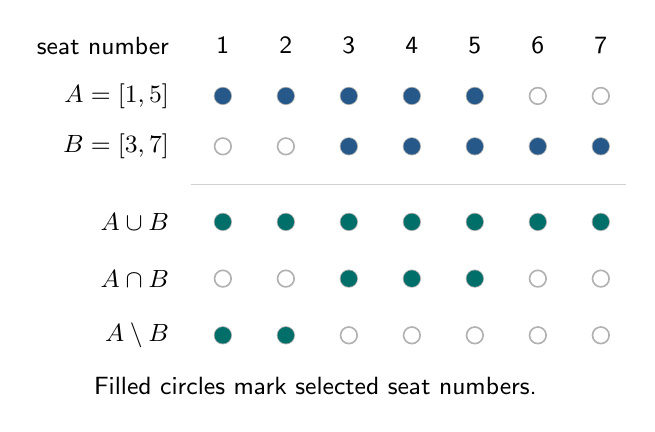
\begin{tikzpicture}[x=0.8cm,y=0.8cm,font=\sffamily\small]
  \definecolor{inputcolor}{RGB}{38,89,137}
  \definecolor{resultcolor}{RGB}{0,111,106}

  \node[anchor=east] at (0.3,5.4) {seat number};
  \foreach \seat in {1,...,7} {
    \node at (\seat,5.4) {\seat};
  }

  \node[anchor=east] at (0.3,4.6) {$A = [1,5]$};
  \node[anchor=east] at (0.3,3.8) {$B = [3,7]$};
  \node[anchor=east] at (0.3,2.6) {$A \cup B$};
  \node[anchor=east] at (0.3,1.7) {$A \cap B$};
  \node[anchor=east] at (0.3,0.8) {$A \setminus B$};

  % Each circle is a numbered seat, not a continuous interval boundary.
  \foreach \row in {4.6,3.8,2.6,1.7,0.8} {
    \foreach \seat in {1,...,7} {
      \draw[gray!60,line width=0.6pt] (\seat,\row) circle[radius=3pt];
    }
  }

  \foreach \seat in {1,...,5} {
    \fill[inputcolor] (\seat,4.6) circle[radius=3pt];
  }
  \foreach \seat in {3,...,7} {
    \fill[inputcolor] (\seat,3.8) circle[radius=3pt];
  }

  \draw[gray!35] (0.5,3.2) -- (7.4,3.2);

  \foreach \seat in {1,...,7} {
    \fill[resultcolor] (\seat,2.6) circle[radius=3pt];
  }
  \foreach \seat in {3,...,5} {
    \fill[resultcolor] (\seat,1.7) circle[radius=3pt];
  }
  \foreach \seat in {1,2} {
    \fill[resultcolor] (\seat,0.8) circle[radius=3pt];
  }

  \node[anchor=west] at (-1.2,0) {Filled circles mark selected seat numbers.};
\end{tikzpicture}
\end{document}
